\pagestyle{fancy}
\lhead{}
\renewcommand{\chaptermark}[1]{\markboth{\thechapter.\ #1}{}}

\chapter{Building blocks}
\label{ch:PhotonicCircuits}
The most important building blocks for developing all-optical switches are:


\section{Waveguides}

To route light in photonic integrated circuits there are different types of waveguides:

\begin{figure}[h]
    \centering
    \includegraphics[width=0.49\textwidth]{strip3d2}
    \includegraphics[width=0.49\textwidth]{rib3d}
    \caption{The strip (left) confines more the light than the rib waveguide (right). However, in the strip, the mode sees more sidewall roughness created during the etching process and usually has higher loss.}
    \label{fig:ribStripSchematics}
\end{figure}


\begin{itemize}
 \item In \textbf{Strip} waveguides, the silicon is fully etched at both sides. This maximizes the lateral index contrast, allowing very tight bends and small footprints. Sidewall roughness is the main source of loss, which is usually in the range of few dB/cm for $220 \times 500$~nm waveguides.

 \item In \textbf{Rib} waveguides, a silicon slab remains at the bottom, where the mode expands. The index difference and confinement factor are smaller than the strip case, requiring higher bending radius. However they can achieve lower loss and allow the introduction of an electrical signal from both sides of the slab, as for example in modulators.
 
 \item If a thin layer of low-index material is inserted in the middle of the core of a strip waveguide, that is called a \textbf{slot} waveguide. These waveguides are interesting for some applications because the mode with polarization perpendicular to the slot layer undergoes a strong field enhancement due to the dielectric constant discontinuity. The orientation of the slot layer can be either horizontal or vertical.
 For sensing, a vertical slot is very interesting, as the slot can be filled with the analyte, whereas for nonlinear applications the horizontal slot has lower loss and therefore longer effective length of the nonlinear interaction.
\end{itemize}


\begin{figure}[h]
    \centering
    \includegraphics[width=0.49\textwidth]{sloth}
    \includegraphics[width=0.49\textwidth]{slotv}
    \caption{The slot can be filled with an analyte (sensors) or a nonlinear material (silicon nanocrystals) and can be horizontal or vertical.}
    \label{fig:slotSchematic}
\end{figure}


There are several methods to calculate the modes in a waveguide (Appendix~\ref{ch:simulations}).
All of them calculate the possible modes that can propagate inside the waveguide, together with its propagation constant and effective index.
Moreover light can travel with two different orthogonal polarization states, quasi transverse-electric (quasi-TE) and quasi transverse-magnetic (quasi-TM), that we refer as TE and TM for simplicity.


\begin{figure}[h]
    \centering
    \includegraphics[width=0.49\textwidth]{te0}
    \includegraphics[width=0.49\textwidth]{tm0}
    \caption{Fundamental transverse-electric TE (left) and magnetic TM (right) modes of a $220\times500~$nm silicon strip waveguide surrounded by silica. In both cases we plot the highest component of the electrical field, which is the horizontal component for TE (Ex) and the vertical (Ey) for TM at 1.55~$\mu$m.}
    \label{fig:modesStrip}
\end{figure}


\begin{figure}[h]
    \centering
    \includegraphics[width=0.49\textwidth]{te0rib}
    \includegraphics[width=0.49\textwidth]{tm0Slot}
    \caption{Left: Fundamental TE mode of a $220\times500~$nm silicon rib waveguide with a 100~nm silicon slab. Right: Fundamental TM mode of a slot waveguide that consists of two $220\times500~$nm silicon slabs separated by a 100~nm silica slot. We can see that the mode expands in the 120~nm slab of the rib waveguide (left) and that the 100~nm silica slot confines the mode inside the slot thanks to the field enhancement discontinuity of both silicon slabs (right). In both cases we plot the highest component of the electrical field, which is the horizontal component for TE (Ex) and the vertical (Ey) for TM at 1.55~$\mu$m}
    \label{fig:modesRibSlot}
\end{figure}


\begin{figure}[h]
    \centering
    \includegraphics[width=0.7\textwidth]{modesSilicon}
    \caption{Effective index for different modes and waveguide widths of a 220~nm height Silicon strip waveguide. The graph shows the guided modes that can propagate inside the waveguide, whose index is above the refractive index of the Silica (1.44).}
    \label{fig:modesSilicon}
\end{figure}


\section{Bends}
Bend waveguides are necessary in all photonic circuits, specially for designing ring resonators and connecting different components. It is therefore of utmost importance to understand light propagation inside the bend.
Bent modes can be calculated using standard mode solvers using a conformal transformation of the index profile as explained in~\cite{Heiblum:75}.
The bend introduces an asymmetry in the mode profile, which can be modeled with a good approximation as an index increase towards the outer side of the bend. This effect pushes the mode to the outer part of the bend, and bend loss occurs in form of radiation losses.

However, Silicon waveguides allow very small bending radius thanks to the high refractive index between the silicon core (3.47) and silica cladding (1.44), enabling high scale integration of photonic integrated circuits. In Fig.~\ref{fig:90bendLoss} we can see that for a strip waveguide with 5~$\mu$m bending radius, losses are lower than 0.04~dB per 90$^\circ$ turn.

\begin{figure}[h]
    \centering
    \includegraphics[width=1.0\textwidth]{bendModes015}
    \caption{1.55~$\mu$m TE Computed mode of a $220\times500~$nm strip waveguide with no bend (left), 5~$\mu$m (center) and 1~$\mu$m (right) bending radius, where the leaking of the mode to the cladding increases significantly.}
    \label{fig:bendLoss015}
\end{figure}


\begin{figure}[h]
    \centering
    \includegraphics[width=0.6\textwidth]{bendRadius_silicon_bp_2d_0p45_TE_2p85deltaN}
    \caption{Simulated losses of a 90$^\circ$ bend for different bending radius. As we can see, strip waveguides allow very small bending radius thanks to the high confinement of the mode inside the Silicon.}
    \label{fig:90bendLoss}
\end{figure}

\section{Fiber to chip coupling}
Coupling between integrated circuits and optical fibers is a serious challenge because of their mode size mismatch. There two main approaches to solve this problem:

\begin{itemize}
 \item Using a \textbf{grating coupler} to couple light from a fiber into the chip~\cite{1017613} allows device testing directly from the wafer. It is based on a resonant structure and must be designed for a certain polarization and wavelength range.
 
 \item We can couple light \textbf{horizontally} with a taper that adapts the mode size from the chip to the fiber. %inside the waveguide to match the mode of the fiber.
 A regular taper only expands the mode horizontally, while an inverse taper narrows the mode first and then it expands in both directions with a more uniform shape.
 Inverse tapers increase the coupling efficiency, but are more sensitive to fabrication tolerances~\cite{Shoji:02}.
 
\end{itemize}



\section{Mach Zehnder interferometer (MZI)}
It is the most basic interferometric structure.
An input beam is divided into two arms with different length or different phase shifts, so the relative phase shift between both arms changes for different wavelengths, interfering either constructive or destructively. The output field is:

\begin{equation}
	E_{out}/E_{in}=cos(\Delta \phi)
\end{equation} 

Where $\Delta \phi$ is the phase difference between both arms of the interferometer, that can be due to different arm length ($\Delta \phi = \beta \Delta L$) or different propagation constant ($\beta$) in each arm ($\Delta \phi = \Delta \beta L$).

\begin{figure}[htb]
    \centering
    \includegraphics[width=0.5\textwidth]{mzi-crop}
    \caption{Schematic MZI interferometer. We can use it as a logic gate by accessing both arms independently, as in Chapter~\ref{ch:paperLogicGates} paper.}
    \label{fig:mziSchematic}
\end{figure}


\begin{figure}[htb]
    \centering
    \includegraphics[width=1.0\textwidth]{mzi13mm350um}
      \caption{Impulse response (top) and transfer function (bottom) measurements of a 350~$\mu$m arm difference MZI (5~ps) using an Optical Vector Analyzer (OVA) (Appendix~\ref{ch:method}). From the Inverse Fourier Transform of the spectrum we can measure the delay between both arms.}
    \label{fig:mzi13mm350um}
\end{figure}


\begin{figure}[htb]
    \centering
    \includegraphics[width=0.35\textwidth,angle=-90]{mziOn} \includegraphics[width=0.35\textwidth,angle=-90]{mziOff}
      \caption{MZI interferometer with constructive (left) and destructive (right) interference.}
    \label{fig:mziOnOff}
\end{figure}



\section{Ring resonators}
Ring resonators are very useful components for filtering, multiplexing, switching and modulating.
An optical ring resonator is a structure formed connecting the input of a directional coupler to one of the outputs (Fig.~\ref{fig:ringSchematic}).
When we couple light of a certain wavelength into the ring, it generates constructive or destructive interference in the multiple turns, so only the wavelengths that satisfy the resonance condition remain inside the ring, which are multiples of the ring length.
The rest of the wavelengths accumulate different phase shifts along the ring and interfere destructively.

\begin{figure}[htb]
    \centering
    \includegraphics[width=0.5\textwidth]{ring}
    \caption{A is the single pass amplitude transmission and k/t the (cross/self)-coupling coefficient of the ring.}
    \label{fig:ringSchematic}
\end{figure}

The transmission equation of a ring can be easily obtained. If we consider an input field $E_{in}$, the first contribution at the output is $E_{in} t$ being $t$ the transmission in the coupler (Fig.~\ref{fig:ringSchematic}).
The second contribution ($-E_{in} k^2$) has the ring single pass amplitude transmission ($A=|A| e^{j\phi}$), two coupling coefficients ($k^2$) and a negative sign due to the $\pi/2$ shift to enter the ring and another $\pi/2$ phase shift to go back into the waveguide.

\begin{equation}
	E_{out}=E_{in}[t-k^2A-k^2tA^2 + \ldots]
\end{equation} 

\begin{equation}
	E_{out}/E_{in}=t-k^2A[1+tA + (tA)^2 +  \ldots]
\end{equation} 

Where the sum of the infinite terms of a geometric progression of common ratio $tA<1$ is $ S_\infty = \frac{1}{1-tA} $

\begin{equation}
	E_{out}/E_{in}=t-k^2A\frac{1}{1-tA}
\end{equation} 

\begin{equation}
	E_{out}/E_{in}=\frac{t-t^2A-K^2A}{1-tA}
\end{equation} 

And we know that $k^2+t^2=1$, so we can substitute $k^2=1-t^2$:

\begin{equation}
	E_{out}/E_{in}=\frac{t-A}{1-tA}
\label{eq:transmissionRing}
\end{equation}

Where the single pass amplitude transmission ($A=|A| e^{j\phi}$) in resonance ($\phi=\beta L=2\pi \frac{ n_{eff}}{\lambda} 2 \pi R= 0,2\pi,4\pi,\ldots$), only has the losses term ($A=\alpha$).
Depending on the relation between the coupling coefficient and the losses, a ring resonator is:

\begin{itemize}
\item \textbf{Under-coupled ($t>A$):}  The coupling is lower than the attenuation in a single trip through the ring. With zero phase at the resonances, each resonance produces a phase fluctuation. 

\item \textbf{Critically coupled ($t=A$):} The attenuation in one trip through the ring equals the coupling coefficient. In this case there is zero transmission at resonance, because the output light coming from the ring and from the input port cancel out.
 
\item \textbf{Over-coupled ($t<A$):} The coupling coefficient is higher than the attenuation through the ring. Therefore the phase accumulates an extra $2\pi$ at each resonance because at the output, more energy is coming from the ring than from the input port, generating an extra phase delay. The phase at the resonance is $\pi$.
\end{itemize}


% \begin{figure}[htb]
%     \centering
%     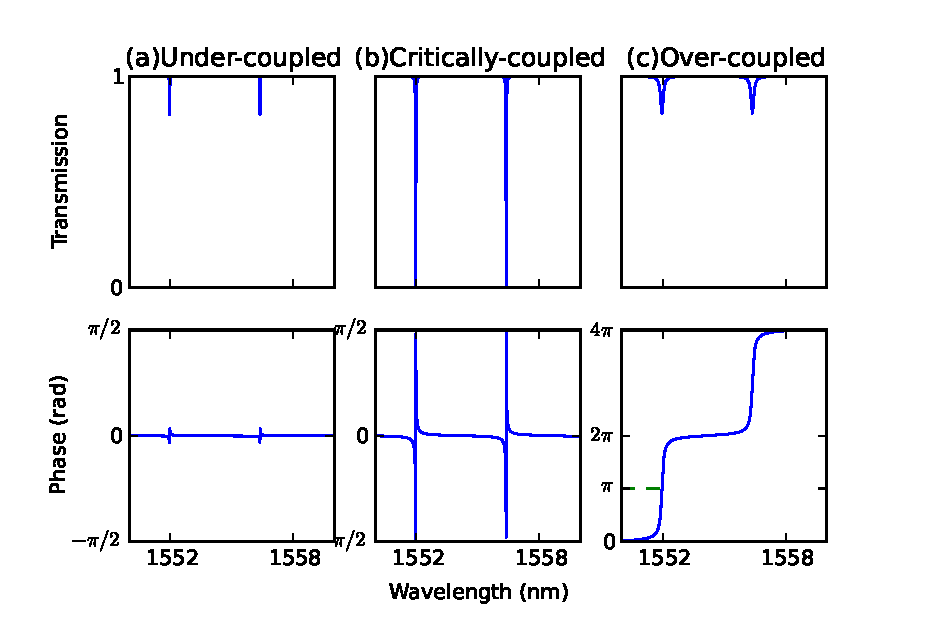
\includegraphics[width=1.0\textwidth]{ringCouplingRegimes}
%     \caption{Simulated transmission and phase spectra of a ring resonator under different coupling regimes.
%     A= 0.99 in all cases, and $t$ is 0.999, 0.99, 0.9 in the left, center and right panels respectively.
%     Distinguishing over- from under-coupling regimes requires the phase response.}
%     \label{fig:ringDifferentCouplingTesis}
% \end{figure}


Rings have a certain free spectral range (FSR), extinction ratio (ER), and resonance full-width half maximum (FWHM), related to the quality factor (Q) and finesse ($F$). These parameters depend not only on the coupling (k) and the amplitude transmission inside the ring (A), but also on manufacturing tolerances~\cite{Bogaerts:12}.

\begin{equation}
	FSR=\frac{\lambda_{res}^2}{n_gL}
\end{equation} 

Where $n_g$ is the group index and $\lambda_{res}$ is the resonant wavelength.

\begin{equation}
	Q=mF=m\frac{FSR}{FWHM}
\end{equation} 

% \begin{figure}[htb]
%     \centering
%     \includegraphics[width=1.0\textwidth]{r20g280TMP13f}
%       \caption{Impulse response (top) and transfer function (bottom) measurements of a 20~$\mu$m radius ring resonator with 280~nm gap and transverse-magnetic (TM) polarization. From the separation between the resonances (FSR) we can extract the group index ($n_g=4.33$).}
%     \label{fig:r20g280TMP13f}
% \end{figure}


$McKinnon~et~al$~\cite{McKinnon2009} develop a method for extracting the coupling and loss coefficients.
However, their formulas do not distinguish which coefficient is loss and which is coupling, so in paper~\ref{ch:paperPhase} we propose a novel experimental technique able to distinguish unambiguously the parameters of the ring. %citaPaperJSQTE
Moreover, when working with very high quality factors ($Q>10k$), backscattering effects can greatly alter the shape to the resonances, so in paper~\ref{ch:paperBackscattering} we present a theoretical model that considers backscattering effects and experimental measurements that demonstrate its validity~\cite{Ballesteros2011}.

% A ring resonator is a very interesting structure for all-optical switching.
% As we want to switch a signal using a control signal, both of them need to satisfy the resonance condition so they can enter the ring and interact in the multiple turns inside the ring.

% \subsection*{MZI as a Logic gate}
% If we access only one of the arms of the Mach Zehnder interferometer we can use it as a logic gate.
% As the data signals will be affecting only one of the branches of the interferometer we can imbalance the interferometer inducing a phase shift through cross-phase modulation (XPM).
% So if the working point is set to a minimum of the MZI, we will have signal at the output (a logic one) with only one of the branches is unbalanced, working as a exclusive OR (XOR).
% Different logic gates can also be achieved modifying the control and data ports.
% 
% 
% \begin{figure}[htb]
%     \centering
%     \includegraphics[width=0.5\textwidth]{logicGate7}
%     \caption{Schematic optical logic gate based on a MZI interferometer.
%     We can induce phase shifts in each arm through cross-absorption modulation (XPM).}%We can filter out data~1 and data~2 using ring resonators at the end of each arm (purple) or at the output.
%     \label{fig:logicGate}
% \end{figure}
% 
% \begin{table}[h]
% \centering
% \begin{tabular}{|c|c|c|} \hline
% \textbf{A} & \textbf{B} & \textbf{A XOR B}\\ \hline
% 0 & 0 & 0\\
% 0 & 1 & 1\\
% 1 & 0 & 1\\
% 1 & 1 & 0\\
% \hline
% \end{tabular}
% \caption{Truth table of a XOR logic gate.}
% \label{table:resultsImGamma}
% \end{table}



\pagestyle{plain}
\bibliographystyle{unsrt}
\bibliography{library}
